% ==================================================
% CHAPTER 6: Using x-rays to measure relative strip position offsets
% ==================================================

\chapter{Using x-rays to measure relative strip position offsets}
\label{chap:xray}

This chapter describes the analysis of x-ray data to measure relative local strip position offsets, which can be compared with results obtained using cosmic data. The reader is referred to the paper describing the x-ray method~\cite{lefebvre_precision_2020}. Some minor changes to the experimental setup have been made since the paper was written. The experimental setup described here is current and was used to collect the data presented in this thesis.
% Makesure to put this in the statement of contribution

% NOTE: Wrote this with information available in JINST, or things I know to be updated (eg. brass holder and collimator). I can guess at other things based on the WedgeAlignment-Production code, but don't actually know. Those things are in iffalse statements.
% --------------------------------------------------
\section{Experimental setup}
% --------------------------------------------------

The x-ray tests were performed after the quadruplets had arrived at CERN, had been were assembled into wedges, and the alignment platforms installed. An x-ray gun was attached to one of the alignment platforms glued to the surface of the wedge and the x-ray beam profile was recorded by the strip electrodes.

\begin{figure}[t]
    \centering
    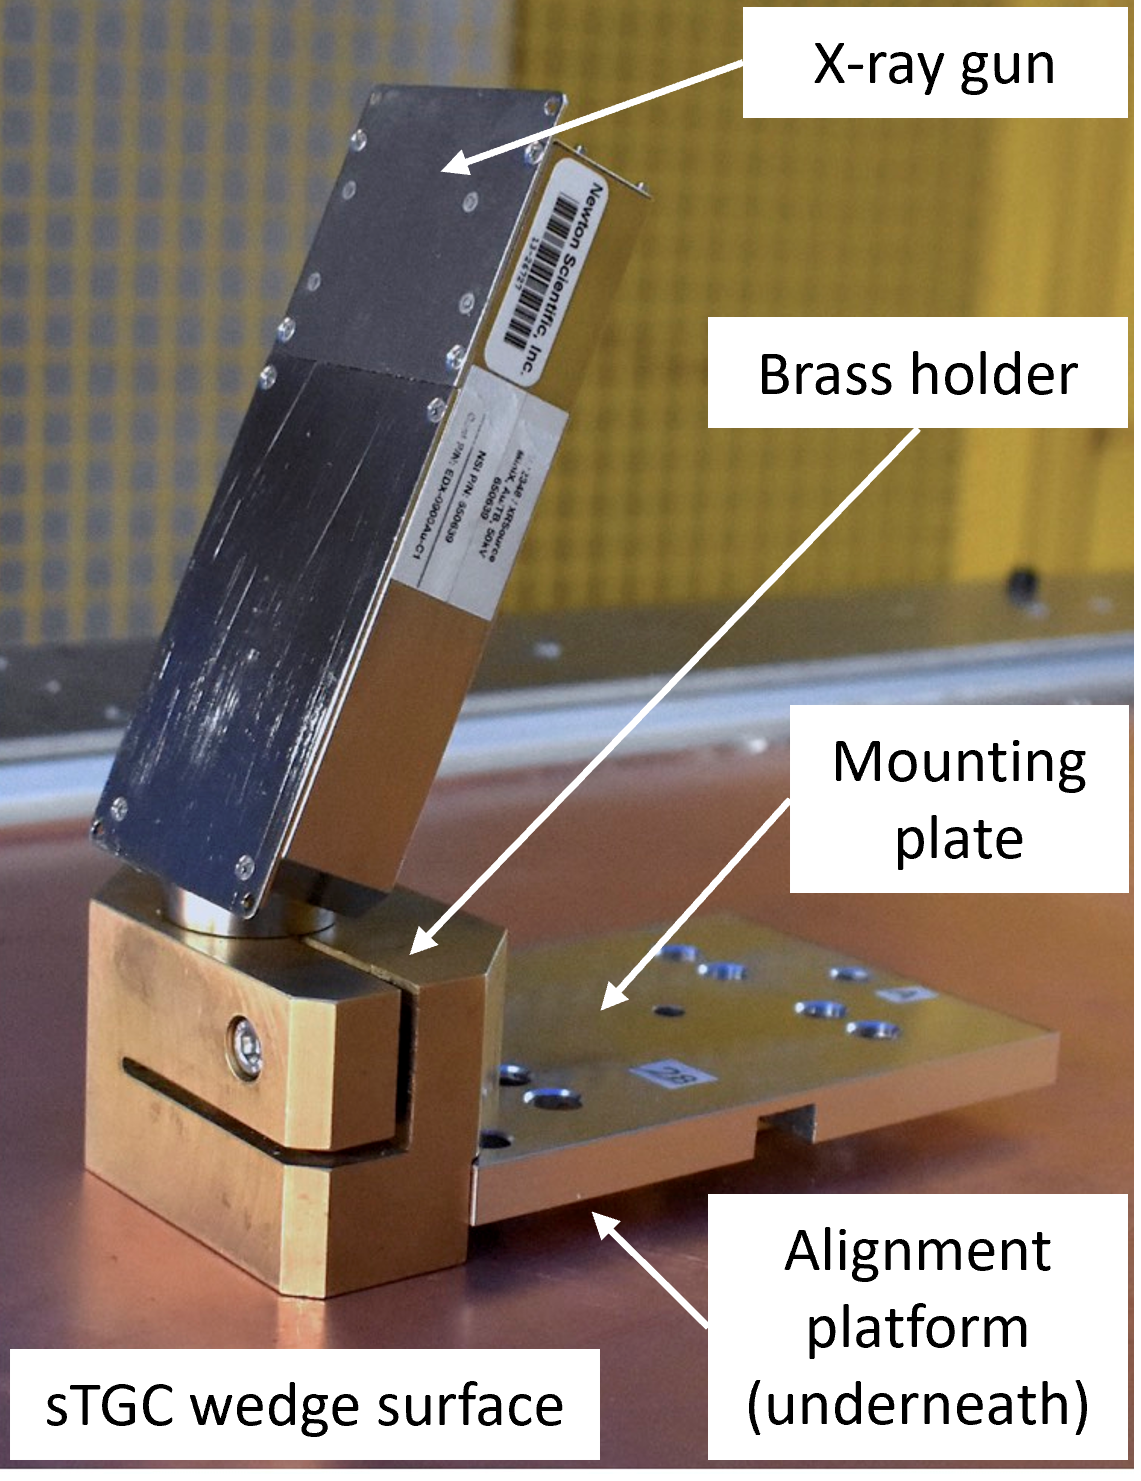
\includegraphics[width = 0.5\textwidth]{figures/xray_setup.png}
    \caption{The x-ray gun mounted to an alignment platform on the surface of  a sTGC wedge. Adapted from~\cite{lefebvre_precision_2020}.}
    \label{fig:xray_setup}
\end{figure}

The sTGC wedges were installed on carts that could rotate their surface to a horizontal position. A mounting platform was installed on top of the alignment platform using a three-ball mount. The x-ray gun used was an Amptek Mini-X tube~\cite{xray_gun}. The x-ray gun was placed in a brass holder with built-in \SI{2}{mm} collimator and \SI{280}{\micro\meter} copper filter. The holder was mounted on one of five positions on the mounting platform, as shown in figure~\ref{fig:xray_setup}. The x-ray gun positions were chosen to avoid wire support structures in the sTGCs that reduce hit efficiency~\cite{lefebvre_thesis} and boundaries between sets of strips read out by two different ASICs that could each have different thresholds. 

As with cosmics data collection, each sTGC also needed gas and high voltage to operate. Each sTGC layer was operated at \SI{2.925}{kV} with high voltage from a NIM crate. The sTGC gas volumes were flushed with CO$_2$ before and during data collection. The sTGCs were not operated using the nominal pentane-CO$_2$ gas mixture due to constraints in its availability based on safety concerns. The sTGC efficiency is significantly lower when operated with only CO$_2$.

% The copper filter helped to reduce the effect of attenuation non-uniformities.
The gun produced x-rays with energies under \SI{40}{\kilo\electronvolt} with peaks in the 7-\SI{15}{keV} range. Peaks in the 0-\SI{30}{keV} range were filtered out by the copper filter and the copper of the sTGCs. The x-rays mostly interacted with the sTGC wedge's copper electrodes and gold-plated tungsten wires via the photoelectric effect. The resulting photoelectrons that enter the gas volume caused ionization avalanches which were picked up by the readout strips.
% During ATLAS operation, the position of the source plates will be monitored using the new alignment system~\cite{nsw_tdr}. Therefore, their position will be known in the absolute ATLAS coordinate system. 

% --------------------------------------------------
\section{Data acquisition}
% --------------------------------------------------

A different version of the same front end electronics, but the same ASIC, as used in cosmics testing were used for the x-ray testing to measure the peak signal amplitude. Data was collected for two minutes per gun position with random triggers. A trigger recorded all signals above threshold. \iffalse within \SI{75}{ns} and the signals on neighbouring strips.\fi  Pad and wire data was not recorded.
% Neighbour triggering based on my understanding of the analysis. Does not actually matter for these purposes.

% --------------------------------------------------
\section{Data preparation}
% --------------------------------------------------

Following a similar approach to the cosmics data analysis described in chapter~\ref{chap:cosmics}, a default pedestal is subtracted from the signal peak amplitude on each electrode.

Clusters are defined as groups of contiguous strip hits recorded within \SI{75}{ns}. The distribution of peak signal amplitude from continuous strip hits is fitted with a Gaussian function, and the mean of the fitted Gaussian is taken as the cluster position. Cluster positions are corrected for differential non linearity (or DNL, see definition in appendix~\ref{appendix:systematics_dnl}). Although the impact of the DNL correction on the reconstructed cluster means is small, it is important to improve the spatial resolution of the sTGC strip layer. Only clusters composed of hits on 3-5 strips are used in the x-ray analysis. Clusters with signal on more than five strips are cut because they were most likely caused by photoelectrons ejected with enough energy to cause more primary ionization and subsequent avalanches as $\delta$-rays.

The x-ray analysis diverges entirely from the cosmics analysis algorithm here because the ionization from x-rays does not originate from one charged particle traversing all layers of a sTGC quadruplet, so there is no track to rebuild. Rather, ionization avalanches~\cite{townsend_electricity_1915} are generated by photoelectrons liberated from the metals of the sTGCs, which only travel through one gas volume and are produced at all angles. Instead of reconstructing a straight line trajectory through multiple sTGC layers, the cluster position distribution on each sTGC layer is used to reconstruct the beam profile. A typical x-ray beam profile is shown in figure~\ref{fig:xray_beam_profile}.

\begin{figure}[t]
    \centering
    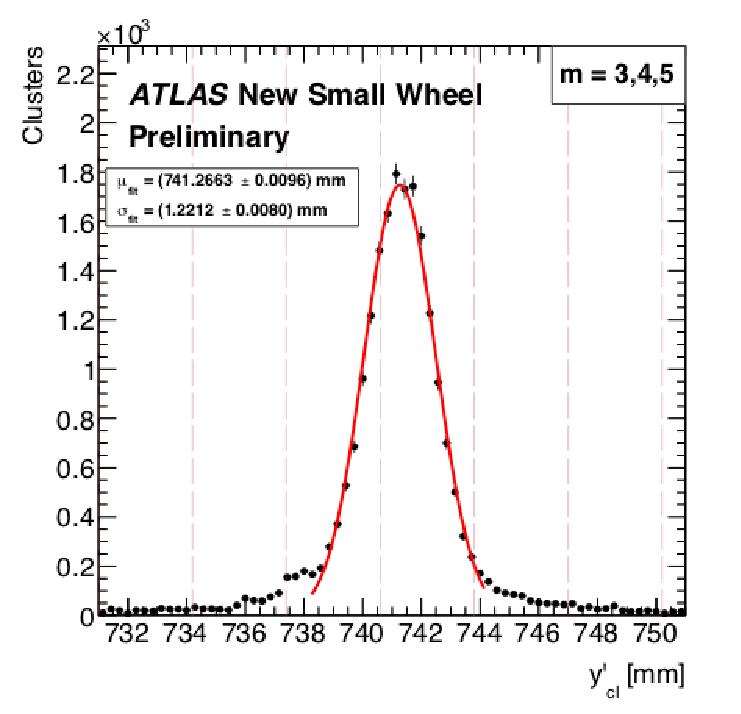
\includegraphics[width = 0.5\textwidth]{figures/figure_xray_beam_profile.pdf}
    \caption{An example distribution of x-ray cluster mean positions after the analysis selection cuts and DNL corrections are applied. The strip cluster multiplicity, $m$, was limited to 3, 4 or 5. The red curve is a Gaussian fit of the distribution and the pink dashed lines denote the edges of the strips~\cite{lefebvre_precision_2020}.}
    \label{fig:xray_beam_profile}
\end{figure}

% --------------------------------------------------
\section{Measuring local offsets}
% --------------------------------------------------
The fitted Gaussian mean of the cluster position distribution is taken as the reconstructed center of the x-ray beam profile on each sTGC layer. The reconstructed center is compared to the expected beam profile center, calculated in two steps. First, the position of the alignment platform with respect to the brass inserts and the nominal position of the strips under the gun position with respect to the brass inserts are used to calculate the expected beam profile center assuming a nominal quadruplet geometry. Second, the expected beam profile center is corrected for the geometry of the brass holder, the positioning and angle of the alignment platforms, and the beam angle. The difference between the expected and reconstructed beam profile centers is a measure of the local offset of the strip electrode pattern. Applying the logic of equation~\ref{eqn:local_translation} to the beam profile, the Gaussian mean of cluster positions on the given layer acts as the recorded position, $y_i$, the expected center is $y_{nom, i}$ and the local offset is $d_{local, i}$ as before, where $i$ denotes the layer. Since the position of the alignment platforms will be monitored continuously by the alignment system in ATLAS~\cite{nsw_tdr}, the position of the strips that should have been at the x-ray gun position are shifted by $d_{local, i}$ and so their absolute positions in the ATLAS coordinate system are known for every position where x-ray data was recorded. Therefore, the x-ray local offsets can be used to measure the position of some strips in the ATLAS coordinate system, as is required for the triggering and precision tracking goals of the NSWs as discussed in chapter~\ref{chap:nsw}.

Studies of systematic effects on the measured beam profile centers lead the x-ray working group to accept an uncertainty of \SI{120}{\micro\meter} on the beam profile centers. The largest uncertainty comes from the effect of the gun angle, which proved difficult to measure and correct for. The details and results of the systematics studies have not been published externally. 

The absolute local strip offsets measured using the method described above are not presented here as the author did not conduct this work. However, the author used the {\em absolute} local offsets to calculate {\em relative} local offsets that can be compared to the relative local offsets measured using cosmic muon data.

% --------------------------------------------------
\section{Measuring relative local offsets}
% --------------------------------------------------

The novelty of the x-ray method and the uncertainty in the x-ray local strip position offsets, which greater than the precision to within which the position of the strips would ideally be known, means that the x-ray local offsets should be validated by an independent method. Absolute local offsets measured using x-ray data and relative local offsets measured using cosmics data cannot be compared directly because they are not defined with respect to the same coordinate system: x-ray absolute local offsets are measured in the ATLAS coordinate system while cosmics relative local offsets are defined with respect to a reference frame established by two sTGC layers in a quadruplet. The following describes the method used to calculate relative local strip position offsets from the x-ray local offsets that can be compared to the cosmics relative strip position offsets.

Given that the measured x-ray beam profile centers are systematically affected by local strip position offsets in the same way as the means of the cosmic ray track residual distributions, the x-ray beam profile centers on each sTGC layer are used to reconstruct a straight line in the $y$-$z$ plane using the beam profile centers on two sTGC layers chosen as reference, in a manner similar to the track reconstruction performed with cosmic muon data. The fitted line will be referred to as an abstract track since it is not built from the positions of a single particle passing through the four layers of an sTGC quadruplet like in the case of cosmic muon tracks. A residual is calculated as the difference between the beam profile center on the layer of interest and the polated straight line fitted from two sTGC layers taken as a reference. The beam profile center on the layer of interest acts as $y_{i}$ and the polated track position acts as $y_{track, i}$ in equation~\ref{eqn:residual}.  As with the means of cosmic track residual distributions, the sign convention is such that the x-ray residual is opposite in sign to the relative local offset of the layer of interest with respect to the two fixed layers. 

% ORIG
% The x-ray local offsets were shown to be correlated with the local offsets calculated from the CMM data, but the CMM data does not include the effect of inter-layer misalignments so the degree of correlation measurable was limited. 
%Cosmics data is affected by inter-layer misalignments. Since the local offsets for x-rays and cosmics data are measured in different coordinate systems, they cannot be compared directly. Bringing the cosmics relative local offsets into an absolute coordinate system is impossible; however, the x-ray local offsets can be brought into a relative coordinate system.

%The measured x-ray beam profile centers were systematically affected by local offsets in the same way as the mean cosmics residuals, as modeled by equation \ref{eqn:local_translation}. Therefore, if a 2-layer track is built from the beam profile centers on each layer and the residual calculated on a third layer, that residual should match the local mean cosmics residual. The residual is the difference between the beam profile center on the layer of interest and the polated track position from the beam profile centers recorded on the two fixed layers. The beam profile center on the layer of interest acts as $y_{i}$ and the polated track position acts as $y_{track, i}$ in equation~\ref{eqn:residual}.

%The track referred to here is not an actual track of the x-ray beam. A beam profile center is actually the Gaussian mean of all selected mean cluster positions recorded during the x-ray data taking period, not a single hit of a track. Building an ``abstract'' track was necessary because the x-rays cause signal in the chamber via the photoeffect so there were not individual ``x-ray tracks'' to record. In fact the x-ray data could be collected separately for each layer. Nonetheless, since the effect of local offsets on the beam profile centers was the same as their effect on the cosmics cluster positions the difference in algorithm between x-ray and cosmics analysis was allowed. 

\newpage
\thispagestyle{empty}
\newgeometry{top=0.5in,bottom=0.5in}
\begin{figure}
\centering
\begin{subfigure}{\textwidth}
  \centering
  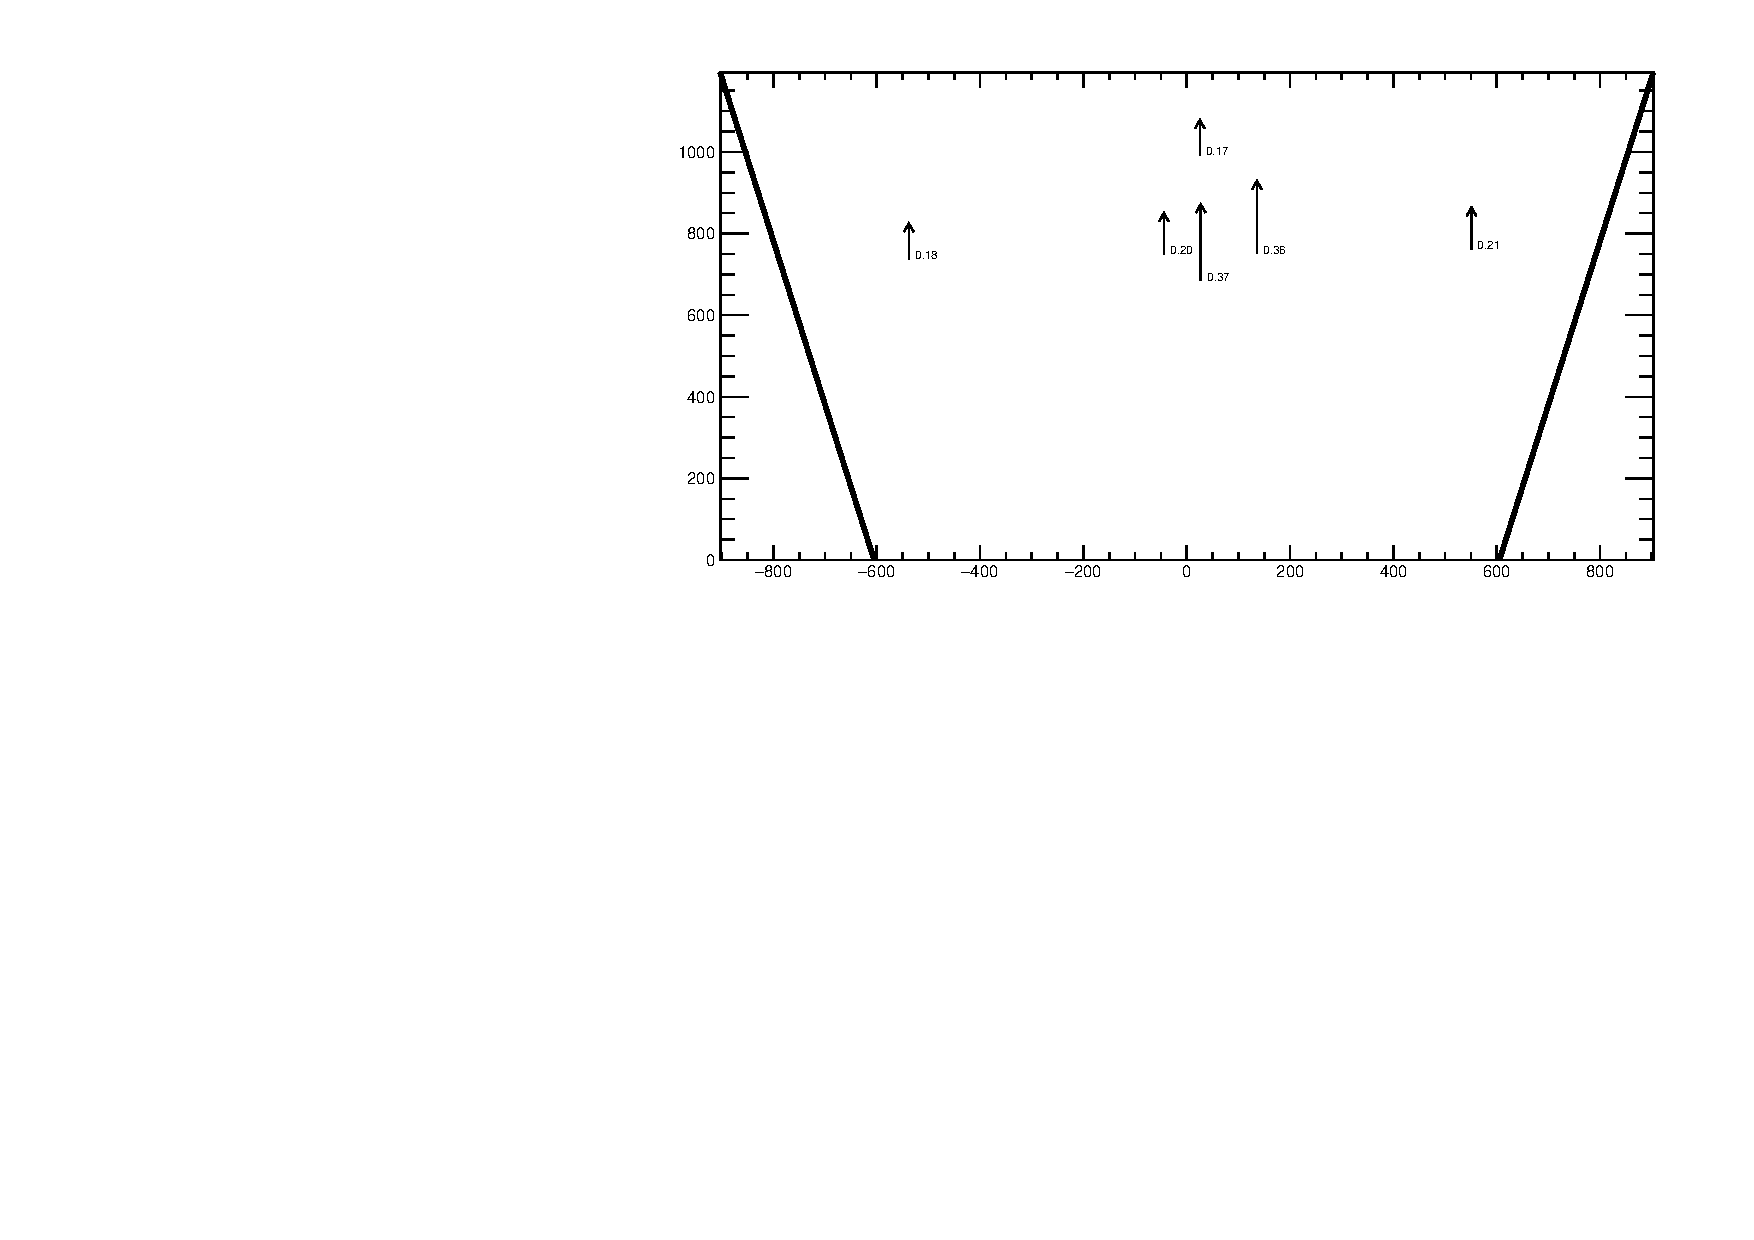
\includegraphics[width=\linewidth]{figures/QL2P11_xray_residuals_layer2_fixedlayers13.pdf}
  \caption{X-ray residuals on quadruplet QL2.P.11 layer 2 obtained using reference layers 1 and 3.}
  \label{fig:xray_res_th2_ql2p11}
\end{subfigure}%
\vspace*{\floatsep}
\begin{subfigure}{\textwidth}
  \centering
  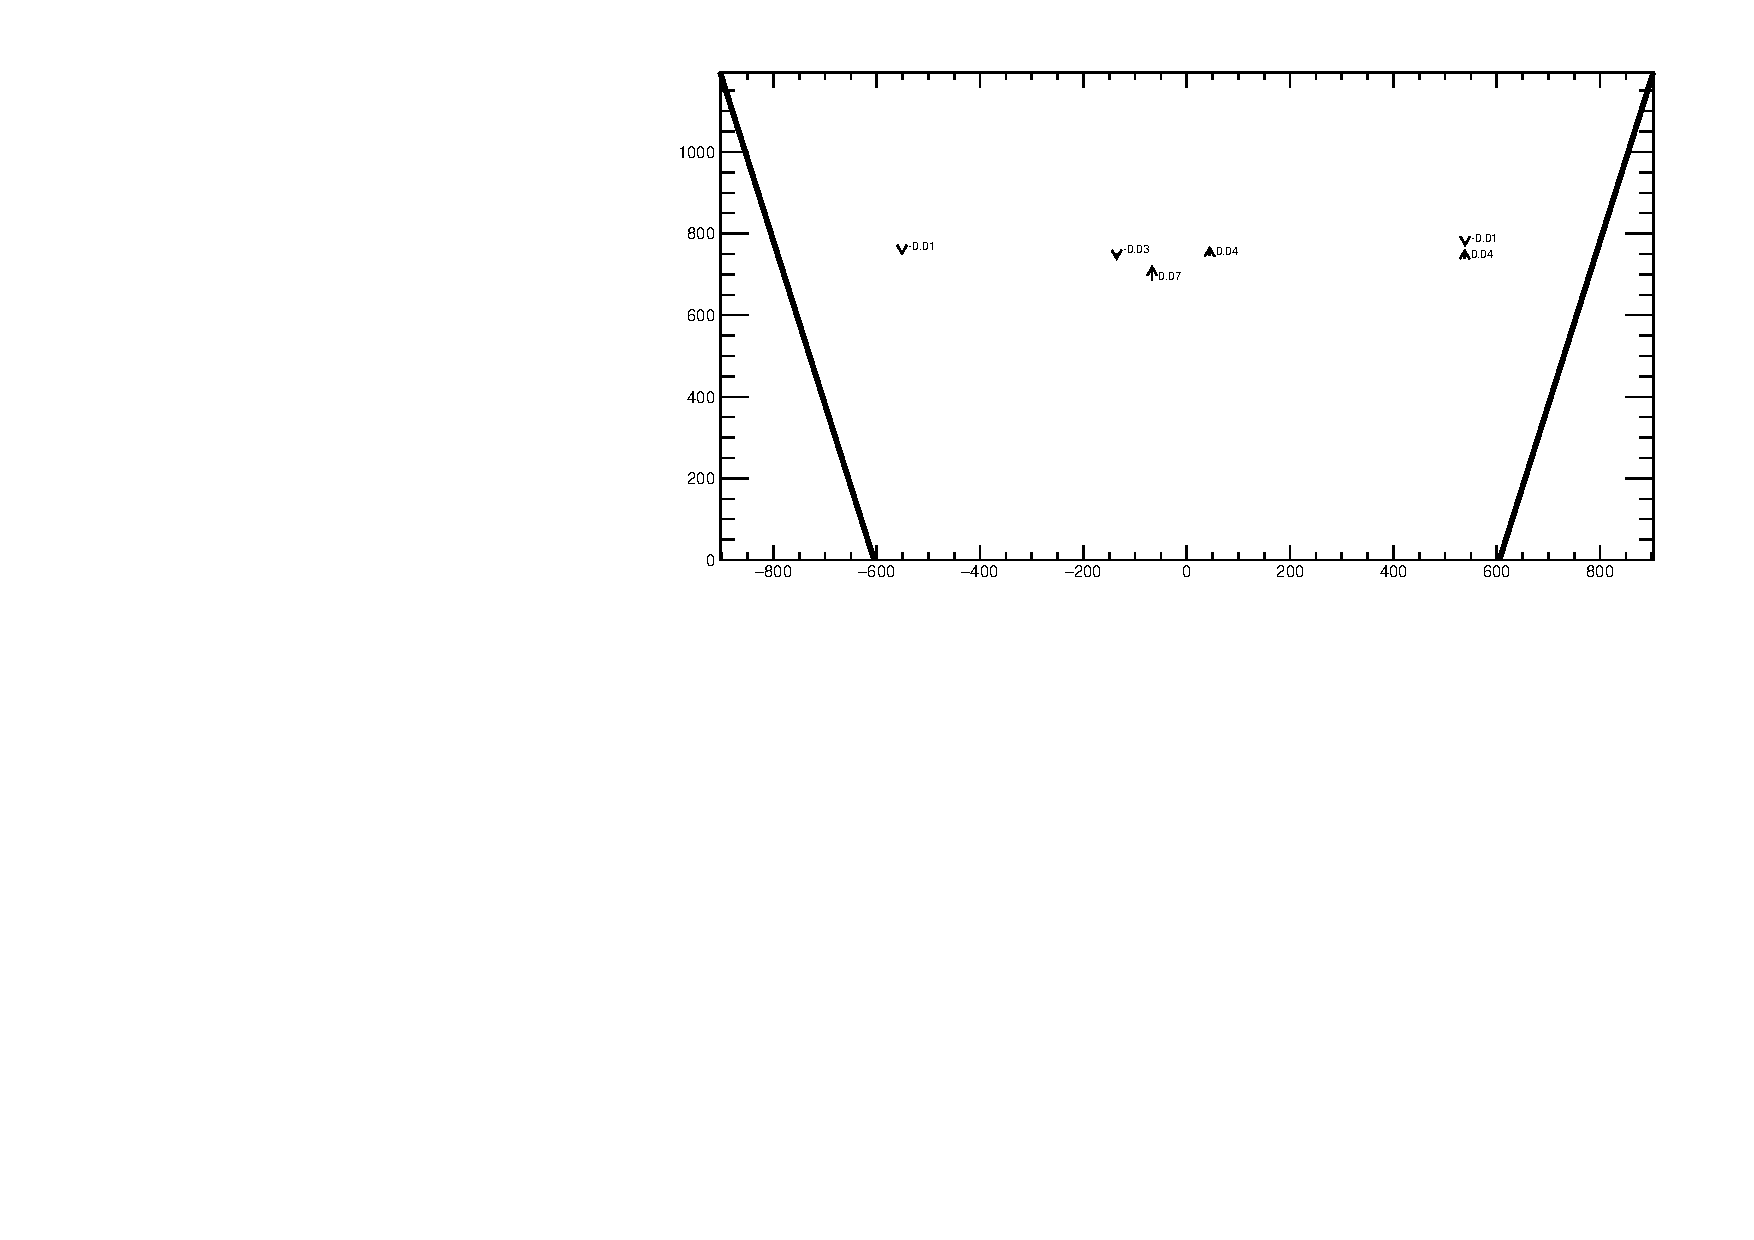
\includegraphics[width=\linewidth]{figures/QL2P08_xray_residuals_layer2_fixedlayers13.pdf}
  \caption{X-ray residuals on quadruplet QL2.P.8 layer 2 obtained using reference layers 1 and 3.}
  \label{fig:xray_res_th2_ql2p8}
\end{subfigure}
\caption{The x-ray residuals on sTGC layer 2 calculated with respect to the beam profile centers on sTGC layers 1 and 3 for quadruplet QL2.P.11 (a) and QL2.P.8 (b). The arrows originate from the expected position of the beam profile center assuming a nominal geometry. The lengths of the arrows are 500 times the value of the x-ray residuals, scaled for visibility. The value of the x-ray residuals are annotated in millimeters and have an uncertainty of $\pm$\SI{0.15}{mm}.}
\label{fig:xray_res_th2}
\end{figure}
\newpage
\restoregeometry

For each x-ray survey position, the x-ray residuals were calculated for all possible pairs of sTGC layers taken as reference and each sTGC layer the straight line could be polated to, as was done for cosmic muon tracks. Calculating a residual required x-ray beam profiles on at least three layers. Figure~\ref{fig:xray_res_th2} shows the x-ray residual values on sTGC layer 2 with respect to reference layers 1 and 3 for sTGC quadruplet modules QL2.P.11 and QL2.P.8.  For module QL2.P.11, a negative relative local offset is measured at all x-ray survey points, indicating a global translation of sTGC layer 2 with respect to layers 1 and 3.

The uncertainty on the x-ray residualsis is obtained by propagating the uncertainty on the reconstructed x-ray beam profile centers (\SI{120}{\micro\meter}) through the polation. The uncertainty on the x-ray residuals ranges from \SI{150}{\micro\meter} to \SI{400}{\micro\meter} from the most to least geometrically-favourable tracking combination. There is no discernible pattern of misalignmnet revealed by the x-ray residuals on QL2.P.8 because they have absolute values smaller than the uncertainty on the x-ray residuals (\SI{150}{\micro\meter}). 

The relative local offsets calculated using cosmics data and x-ray data will be compared in the next chapter.